\chapter{机器学习概述与数据特征工程}
\section{引言}
从本章起,本研究将使用机器学习的一般方法对PE患者及正常妊娠孕妇的脉搏波数据进行相关分析研究。
作为过渡章节,本章首先进行了机器学习的一般概述,介绍了机器学习的一般步骤与流程,并明确本研究的机器学习任务。特别地,
在机器学习开始之前,一般还需对使用的数据进行额外的处理工作,即数据特征工程,本章也对这部分的工作内容进行了相应的介绍。

\section{机器学习概述}
本小节将从机器学习的基本概念、分类、一般步骤流程及本研究涉及的机器学习任务等方面进行介绍。
由于篇幅内容所限,机器学习领域常见的术语并没有在正文中过多提及,其解释可参见本文末附录D。
\subsection{机器学习简介}
一般认为,机器学习是一门致力于研究通过计算的手段、利用已有的经验来改善系统自身性能的学科(和艺术)\cite{Zhou2016,Aurélien2018}。其中,Tom Mitchell对机器学习给出了一种最为经典的形式化定义:
计算机程序利用经验$E$学习任务$T$,其性能是$P$,如果针对任务$T$的性能$P$随着经验$E$不断增长,那么我们就说关于$T$与$P$,该程序对$E$进行了学习,这一过程如\autoref{fig:etp}所示\cite{mitchell1997,Zhou2016}。
对计算机程序而言,$E$通常以数据的形式存在,因此机器学习也可以看成从相关数据中产生模型的算法过程,不显式编程是机器学习最典型的特征。
\begin{figure}[htbp]
  \centering
  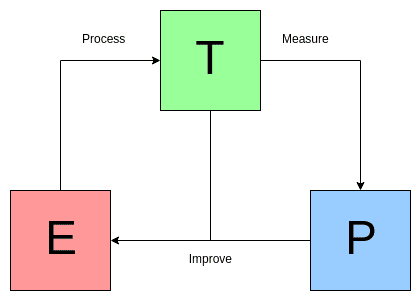
\includegraphics[width=.5\linewidth]{features/etp}
  \caption[机器学习方法的形式化定义]{\label{fig:etp}机器学习的形式化定义}
\end{figure}

尽管机器学习的相关概念早在上世纪五十年代就已经被提出,但直到进入新世纪后,机器学习才真正迎来井喷式发展的黄金期。在过去二十年中,由于半导体电子计算机行业的充分发展,人类收集、传输、处理数据的能力取得了长足的进步,
人类各种社会活动中出现的海量数据具备了能够被挖掘、分析的硬件基础与需要被分析并加以利用的客观需求。在此背景下,机器学习受到了学者们的广泛关注并进入了蓬勃发展阶段,不论是理论基础方面亦或是应用研究方面都
得到了巨大的发展,取得了重大突破。目前,机器学习技术已经被成功应用在模式识别、数据挖掘、自然语言处理、语言识别、图像识别、芯片设计、信息检索及生物信息学等学科领域,
尤其是为交叉学科的发展研究提供了新的技术支撑与突破点\cite{Zhou2016,Aurélien2018,Li2017}。

\subsection{机器学习的分类}
尽管有多种分类标准,一种比较\cite{awad2015,Li2017}。
监督学习、非监督学习、半监督学习、强化学习

\subsection{机器学习的一般步骤}



* 提出具体问题(PE甄别)
* 获取数据(原始PPG->特征提取)
* 研究数据的特性(相关性、有效性,分布特性)
* 数据准备(缺失值、标准化、特征筛选、构建新特征等)
* 探索多种机器学习模型,列出最佳模型
* 超参数调整,优化最佳模型
* 结论与演示,什么有效什么无效,最后结果
* 生产与部署

\begin{figure}[htbp]
  \centering
  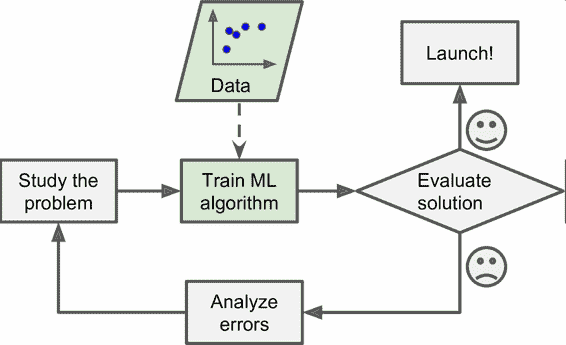
\includegraphics[width=.6\linewidth]{features/ml}
  \caption[机器学习方法]{\label{fig:ml}机器学习方法\cite{Aurélien2018}}
\end{figure}
\subsection{本研究的机器学习任务}
回归到本研究的工作内容上来,不难发现,

探求子痫前期与脉搏波波形之间的潜在关系,

探求子痫前期与孕妇脉搏波数据之间的关系


\section{数据特征工程}
特征的处理

\subsection{数据集构建}
* 分析数据集准备:两种方式

  * A. by pulse

  * B. by person
\subsection{PPG时域描述特征集构建}

本小节对本研究实际采用的多种PPG时域描述特征进行汇总,对各参数符号及前置计算条件也进行了统一说明,如\autoref{tab:allfeatures}所示。
TODO
\begin{center}
    \fontsize{10}{4}
    \begin{longtable}{p{3cm}<{\centering}p{1cm}<{\centering}p{2cm}<{\centering}p{6cm}<{\centering}p{1cm}<{\centering}}
        \caption{本研究使用的所有PPG时域指标一览}\\
        \label{tab:allfeatures}\\
        \hline\hline
            \textbf{研究者}&\textbf{时间}&\textbf{脉搏波参数}&\textbf{研究结果}&\textbf{备注}\\
        \hline
        \endfirsthead
        \caption[]{(续)}\\
        \hline
            \textbf{研究者}&\textbf{时间}&\textbf{脉搏波参数}&\textbf{研究结果}&\textbf{备注}\\
        \hline
        \endhead 
        \hline
        \endfoot
        \hline\hline
        \endlastfoot
        &       &       &       &  \\
        &       &       &       &  \\
        &       &       &       &  \\
        &       &       &       &  \\
        &       &       &       &  \\
    \end{longtable}
\end{center}
\subsection{两种划分方式}
\subsection{数据集的处理}

\subsection{数据清洗}
* 处理缺失值

\subsection{新特征的创建}
* 构建新特征(char参数)
\subsection{相关性验证}
* 分布特性

  * 有无差异性,SPSS统计,已用python实现

  * 特征相关性,heatmap
\subsection{特征缩放}
* 标准化
\subsection{特征降维}
* 降维与特征贡献度

* 部分工作需要下一章节完成后才能确认
\section{小结}